\documentclass{svmult}

\usepackage[utf8x]{inputenc}
%\usepackage{cite}
%\usepackage{graphicx}
\usepackage{makeidx}
\usepackage{multicol}
\usepackage{footmisc}
\usepackage{ucs}
\usepackage{amsmath}
\usepackage{amsfonts}
\usepackage{amssymb}
\usepackage{textcomp}
\usepackage{epstopdf}
\usepackage{natbib}
\usepackage{longtable}
\usepackage[labelfont=bf,labelsep=space,font=small]{caption}
\usepackage{lipsum}

\usepackage[pdftex]{graphicx}
\graphicspath{{./Figures//}}

\begin{document}
\title*{MCDM applied to the partioning problem of 3D-stacked integrated circuits}
\author{N.A.V. Doan, D. Milojevic, Y. De Smet}

\maketitle

\section{Introduction}

In order to continuously improve the performance of integrated circuits (IC), technologists have compelled themselves to follow the well-known Moore's Law (see Figure \ref{fig:mooreslaw}). This empirical law predicts a doubling of the transistors' density each 18 months and therefore increasing logic capacity of the circuit per unit area.

\begin{figure}
\begin{center}
\includegraphics[width=0.7\linewidth]{mooreslaw.png}
\end{center}
\vspace{-0.5cm}
\caption{Moore's law \cite{mooreslawpic}}
\label{fig:mooreslaw}
\end{figure}

The improvements of 2D architectures are primarily driven by the reduction of the transistor size. However, with the miniaturization, quantum effects such as quantum tunnelling will significantly affect how a transistor behave. Indeed, even if a transistor is blocking, current can flow through due to quantum tunnelling such that it will be difficult to control its state and thus the basic working principle of a transistor \cite{1240081}. In addition to these physical aspects, economical considerations that will hinder the IC evolution beyond 20nm have to be taken into account \cite{5227192,PFF10}.

In order to overcome these limitations, new technologies have been proposed such as the carbon nanotubes \cite{tans1998room}, the nanowire transistors \cite{doi:10.1021/nl025875l}, the single-electron transistors \cite{citeulike:4194929}, and also the 3D-Stacked Integrated Circuits (3D-SIC) proposed by the academic and industrial communities. The latter has been often cited as the most prominent one as it is based on the current technologies and still uses silicon as basis material; 3D-SICs can also allow shorter interconnection lengths, smaller footprint, larger bandwidth, heterogeneous circuits among their main advantages \cite{659500,1652906,981091,4299568}.

Fast evolution of IC manufacturing technologies makes even the design of 2D-ICs a complex and tedious task with the growing number of design choices at the system level (e.g. number and type of functional units and memories, type and topology of the interconnection system, etc.) and physical level (respecting area/timing/power constraints). Using 3D-SICs introduces even more degrees of freedom: number of tiers, choices for manufacturing technology (e.g. full 3D integration, silicon interposer, face-to-face, back-to-face, etc.), 3D partitioning and placement strategies etc. These new degrees of freedom will contribute to the combinatorial explosion of already huge design spaces. Moreover, practice and 2D design experience cannot be fully exploited with 3D technology, since 3D-SICs change considerably the way ICs are implemented. Indeed, physical implementation of ICs involves solving several complex problems and hence work only with approximated solutions.

Current design flows can produce workable solutions after manual definition of the physical constraints as there are no preconceived method that can provide good solutions. Also, they are sequential in nature as certain parameters are fixed at certain stages in the flow, which can lead to locally optimal solutions that are far from global optimums so this requires time consuming (hence, costly) iterative processes to adjust these parameters. Since the 3D technology is even more complex than the 2D, it is necessary to improve the current design flows by developing design exploration \cite{PFF10}.

One of the solutions to face this problem is to develop high-level tools which can quickly explore design spaces and give early and reasonably accurate performance estimations based on physical prototyping of the 3D circuits~\cite{PFF10}. In addition, performance estimation/optimization and the selection of the most-suitable solutions usually implies to take several objectives into account (e.g. maximization of the performance, minimization of the cost, minimization of the package size, etc.).

Currently, these high-level design tools can be considered to follow a uni-criterion paradigm. Indeed, they have sequential development steps and each criterion is optimized without considering the impact on other criteria. This can lead to several rollbacks in the design flow since the achievement of the requirements can be time consuming (typical design iterations are measured in weeks). For instance, current tools will only minimize the area of a circuit to reach the timing constraints by solving a 2D place-and-route problem and this will be more complex with 3D-SICs because the system has also to be partitioned.

On the other hand, multi-criteria approaches have been developed to consider all the criteria simultaneously. Designing 3D-SICs inherently implies a huge design space and numerous degrees of freedom and criteria, hence many possible choices when it comes to decide upon the IC to produce. With these reasons, we propose in this work to apply a multi-criteria paradigm with the PROMETHEE methods for the design of 3D-SICs.

\section{Related works}

\subsection{Multi-criteria decision making tools: using the PROMETHEE methods}

In this subsection we recall the basics of the PROMETHEE and GAIA methods. Of course, a detailed description of these approaches goes beyond the scope of this contribution. Therefore we refer the interested reader to \cite{BraMar2005} for a detailed analysis.

Let $\mathcal{A}=\{a_1,a_2,\ldots,a_n\}$ be a set of $n$ alternatives and $\mathcal{F}=\{f_1,f_2,\ldots,f_m\}$ be a set of $m$ criteria. Without loss of generality, we assume that all criteria have to be maximized. The PROMETHEE methods are based on pairwize comparisons. At first, each pair of alternatives $a_i,a_j \in \mathcal{A}$ is compared on every criterion $f_k$:

$$
d_k(a_i,a_j) = f_k(a_i) - f_k(a_j)
$$

The quantity $d_k(a_i,a_j)$ represents the \textit{advantage} of $a_i$ over $a_j$ for criterion $f_k$. On the one hand, when $d_k(a_i,a_j)$ is small enough, there is no good reason to say that $a_i$ is better than $a_j$ regarding criterion $f_k$. On the other hand, when $d_k(a_i,a_j)$ exceeds a certain limit, the decision maker may express that $a_i$ is strictly preferred to $a_j$ for $f_k$. In order to model these statements, the difference $d_k(a_i,a_j)$ is transformed into a unicriterion preference degree, denoted $ P_k(a_i,a_j)$, by using a non-decreasing function $H_k$;

$$
P_k(a_i,a_j) = H_k(d_k(a_i,a_j)), \; \; \forall \; a_i, a_j \; \in \; \mathcal{A}
$$

The quantity $P_k(a_i,a_j) \in [0, 1]$ and $P_k(a_i,a_j)=0$ when $d_k(a_i,a_j) <0$. There are plenty of functions that can be considered to compute the unicriterion preference degrees. In most software implementing the PROMETHEE method, $6$ main functions are considered \cite{Hayez}. Figure \ref{fig:criterion5} represents the so-called linear preference function. Two thresholds characterize it:
\begin{itemize}
\item $q_k$ plays the role of an \textit{indifference} threshold. When the difference $d_k(a_i,a_j) \leq q_k$, it is considered to be so small that the unicriterion preference is equal to zero;
\item $p_k$ plays the role of a \textit{preference} threshold, When the difference $d_k(a_i,a_j) \geq p_k$, it is considered to be important enough to state that $a_i$ is strongly preferred to $a_j$ for this criterion.
\end{itemize}

\begin{figure}[h!]
\begin{center}
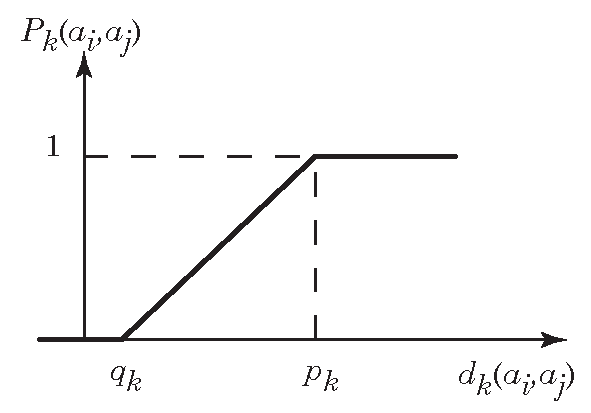
\includegraphics[width=0.7\linewidth]{criterion5.pdf}
\end{center}
\caption{Generalized criterion of type 5}
\label{fig:criterion5}
\end{figure}

Once the unicriterion preference degrees between two actions $a_i$ and $a_j$ have been computed for every criterion, one has to aggregate these marginal contributions to obtain $P(a_i,a_j)$  i.e. a global measure of the preference of $a_i$ over $a_j$:

$$
P(a_i,a_j)= \sum_{k=1}^{m} \omega_k \cdot P_k(a_i,a_j)
$$

where $\omega_k$ represents the relative importance of criterion $f_k$. These weights are assumed to be positive and normalized. Obviously, we have $P(a_i,a_j) \geq 0$ and $P(a_i,a_j) + P(a_j,a_i) \leq 1$.\

The PROMETHEE I and II rankings are based on the exploitation of the matrix $P$. Therefore, three flows are built.; the positive flow $\phi^+$, the negative flow $\phi^-$ and the net flow $\phi$:

$$
\phi^+(a_i)= \frac{1}{n-1} \sum_{a_j \in \mathcal{A}, i \ne j}
P(a_i,a_j)
$$

$$
\phi^-(a_i)= \frac{1}{n-1} \sum_{a_j \in \mathcal{A}, i \ne j}
P(a_j,a_i)
$$

$$
\phi(a_i)=\phi^+(a_i)-\phi^-(a_j)
$$

The PROMETHEE I ranking is obtained as the intersection of the rankings induced by $\phi^+$ and $\phi^-$. The PROMETHEE II ranking is given by the ranking given by $\phi$.

Finally, it is worth noting that:

$$
\phi(a_i) = \frac{1}{n-1} \sum_{k=1}^{m} \sum_{a_j \in \mathcal{A}} {[P_k(a_i,a_j)-P_k(a_j,a_i)]} \cdot \omega_k = \sum_{k=1}^{m} \phi_k(a_i) \cdot \omega_k
$$

where $\phi_k(a_i)$ is called the $k^{th}$ unicriterion net flow assigned to action $a_i$.

The PROMETHEE I and II ranking provide prescriptive tools for decision making. The GAIA \cite{MarBra1988} tool complements them with a descriptive approach. The idea is to represent each alternative by its evaluations in the unicriterion net flow space:

$$
\Phi(a_i)=[\phi_1(a_i),\phi_2(a_i),\ldots,\phi_m(a_i)]
$$

GAIA is the result of a principal component analysis applied on this dataset. Therefore, the decision maker is able to visualize the decision problem on a plane and compare:
\begin{itemize}
\item the relative positions of alternatives (in order to identify groups of similar or distinct alternatives profiles);
\item the relative positions of criteria (in order to identify conflicts or redundancies);
\item the relative positions of alternatives with respect to a given criterion (in order to identify the best and worst alternatives for the different points of views);
\item the relative positions of alternatives with respect to the so-called \textit{decision stick} (in order the identify the best compromise solutions).
\end{itemize}

% Section3: Case study
%!TEX root = ChapSpringer_Main.tex
\section{Case study}
%!TEX root = ChapSpringer_Main.tex
\section{3D integration technology}
3D integration technology is considered to be one of the most promising paths to enable further scaling of Integrated Circuits (ICs). Over the past years many different 3D integration technology flavors have been proposed in both academia and industry. Depending on the integration granularity, a very coarse grain 3D technology classification differentiates between 3D-Stacked Integrated Circuits (3D-SICs) and 3D Monolithic integration. Each of these technology options has it's own merits and drawbacks and as of today there is no clear preference for one or the other. The right choice is very much design dependent and is strongly affected by our ability to perform optimal design implementation.

3D-SICs are built using 2 (or more) fully processed integrated circuits (wafers) that are integrated vertically one on the top of each other (i.e. dies are stacked). Different 3D structures that enable this particular type of 3D integration have been proposed over the past years and they typically include: wire bonding, Through Silicon Vias (TSV), micro-bumps and copper pads. Even if the wire bonding technique is well known, practical usage remained limited because of the connection pitch that is quite high (\~100 micrometer range). Also, wire bonds have high resistance and capacitance that will strongly affect delay and power of a 3D wire. Further, as wire bonds appear at the periphery of the IC, the signals connected to them need to be routed throughout the whole circuit. For all these reasons it is generally considered that the wire bonding is not well suited for efficient 3D integration.

On the other hand TSVs, micro-bumps and copper pads are much more promising technology features since they can be manufactured at very low pitch, the diameter depends on the structure but is generally in the um range allowing dense 3D integration (many inter-die nets). These 3D structures also have good resistance and capacitance values, allowing small delay and power overheads of 3D nets compared to wire bonding and even 2D as long as we enable some wirelength savings for 3D.

With these structures 3D circuits can be stacked in many different ways depending on the orientation of the circuit \emph{face}, i.e. the side of the IC where we find the active layer (transistors i.e. gates). Not all of the options are interesting from the integration perspective, Face-to-Face (F2F) and Face-to-Back (F2B) integration schemes are the ones that are used most of the time. Cross-sections of F2F and F2B 3D integration schemes is shown on Figure~\ref{fig:3D-Stacking}).

\begin{figure}[h!]%
\centering
\includegraphics[width=0.95\columnwidth]{3D_IC.pdf}
\caption{Cross section of Face-to-Back and Face to Face 3D-Stacked Integrated Circuit\label{fig:3D-Stacking}}
\end{figure}

In F2F 3D-SIC, the face of both dies are oriented towards each other and they are interconnected directly. Input/output TSVs are used to connect the active layer of one of the dies to the package ensuring the system communication with the external world. F2F is in principal limited to stacking of two dies only (although it would be possible to stack yet another die on the top of the stack using F2B approach). In case of F2B 3D-SIC, face of one die is oriented towards the back of other die. The active layers of the dies are connected using TSVs, a vertical connection that goes through the substrate of the die. Active layer of one of the dies is exposed to the package used for communication of the system with the external world. F2B can be used to stack more than two dies and is used for manufacturing of highly dense SRAM and DRAM circuits.

The assembly of the dies can be carried out at die or at the wafer level, hence we distinguish: a) Die-to-Die, b) Die-to-Wafer, or c) Wafer-to-Wafer 3D integration. Each assembly method has its advantages (and disadvantages) and the choice depends on the application needs to realize the cost benefits of the 3D integration (trade-off between the wafer processing speed, yield and die area). From the design perspective, there is no significant difference in the choice of assembly approach. We can thus safely assume any of the proposed assembly methods. 3D stacking technology is mature today and is already used in production lines (e.g. DRAM/FLASH memories).

In 3D monolithic integration multiple transistor or logic gate layers are formed sequentially starting from the bottom-most layer. Minimal interconnect structures are used in between these layers: Monolithic Inter-Layer vias (MIVs) for vertical connections and very limited metal layers for horizontal connectivity. The dimension and parasitics of MIVs are of the order of a local via (in the range of nm). As a result, ultra fine-grained vertical integration of devices is possible. The integration grain is finer from the one of the 3D-SICs, since we can stack at lower level (transistor and gate).

If the stacking is happening at the gate-level, the appropriate EDA tools should perform system partitioning at gate-level, and they should be able to place \& route the design in 3D. Note that current EDA tools are not ready for this, since the IC design was a 2D problem until today. If stacking happens at transistor level, the existing EDA, 2D, tools can be used because the problem is now moved to the one of the 3D standard cell design.

While 3D monolithic integration is very promising, there are lot of issues that remain associated with the efficient wafer manufacturing. 3D monolithic process requires high-temperature operations that heavily impact the device performance. Thus, it is known that two consecutive layers will not have the same performance; the top layer having worse performance than the bottom layer, since it is processed afterwards. This will have important consequences on system design and will lower the benefits of such integration.

In the context of this work we focus on 3D-SIC circuits approach.

%!TEX root = ChapSpringer_Main.tex
\subsubsection*{Implementation}
In order to assess physical parameters of an Integrated Circuit (IC) we need to create an IC layout model. In traditional IC design this model is typically generated after gate-level synthesis and place\&route (P\&R). Both steps are performed using Electronic Design Automation (EDA) tools, in a sequence of many different tools. The whole processes typically requires many man and CPU cycles before final model is built. This is due to the system complexity; the accuracy of the models at different abstraction levels that we need to build; and the lack of completely automated methods and algorithms (most of the problems that any design flow is solving are NP-hard problems). To deal with 3D design we have extended the commercially available tools suite from Atrenta (now Synopsis).

The flow is depicted on Figure~\ref{fig:3DFlow}, and we do provide a bit more detailed explanation of each flow step.

\begin{figure}[h!]%
\centering
\includegraphics[width=0.75\columnwidth]{DesignFlow.pdf}
\caption{Sequence of steps required to enable 3D-SIC design (3D Design Flow)\label{fig:3DFlow}}
\end{figure}

\textbf{Step 1: RTL Synthesis} – The input of the proposed flow, as in any IC design flow, consists of several elements. First we need to provide the description of the circuit itself. This is done using any of the standard Hardware Description Languages (VHDL, Verilog). Also, if present, abstracted high-level models of certain blocks cab be supplied with interface definition, area, power, timing etc. (i.e. black-boxes). Finally, typical system constraints (timing) are supplied through standardized file format (.sdc files).

Once the design database is ready, the RTL is synthesized to gate-level netlist using standard technology files (.lib and .lef files) provided by the technology vendor. Note that if the design is intended for 2.5D/3D integration, the technology files will have to capture both electrical and geometrical information not only for standard cells, but also for 3D specific features such as TSVs, micro-bumps, Cu-pads, RDLs, etc. that will be instantiated depending on the stack configuration (F2F or F2B) chosen.

Synthesized gate-level netlist is analyzed for area, timing, logical congestion and other properties. The constraints and synthesis tool guides are adapted to reach realistic goals. Once the synthesis flow is stable i.e. the synthesis process produces the netlist in line with timing constraints, generated netlist can be used as input for both 2D and 3D physical design flows.

\textbf{Step 2: Clustering} – Prior to floorplanning, the gate-level netlist is partitioned into a number of  “reasonably” sized physical clusters of standard cells. The clustering is done so that the floorplan engine works on a reduced number of placeble instances. The size of clusters (the meaning of “reasonable”) will depend on the total circuit size. In general it is chosen in such a way, so that the total number of clusters is in order of few dozens to few hundreds of physical (thus placeble) entities. This is the optimal number of instances (tool run-time vs. quality of the solution) for the floorplan engine.

The purpose of this step is twofold. First, the system is viewed as an assembly of blocks, rather then a collection of logic gates (it could be few dozen of millions) in the design to enable floorplanning (i.e. block level placement) as explained. But secondly, such system view will help in establishing what should go where in the stack.

Standard cell clustering can be performed using many different methods. Note that this is a very important step since the quality of the physical design will depend on the clustering scheme adopted. In the current design flow we can use either top-down approach (from top-level of the design, way to the standard cell level) or bottom-up (from the standard cell level and up). Different clustering objectives could be achieved during clustering: keeping and following the logical hierarchy, creating clusters of the similar size, hierarchical min-cut across the clusters, etc. Note that in the case of the 3D integration, the clustered netlist is further partitioned into a number of gate-level entities (that will remain clustered), equal to the number of dies in the system (see next step, 3D-Partitioning).

\textbf{Step 3: 3D-Partitioning} – This step is performed only in a 3D flow. The stack structure: the number of dies, technology node on per die basis (this is to support heterogeneous integration), stacking orientation (face-up or face-down), 3D structure properties (TSV/ubump/CuPad) and RDL net properties (width/pitch), etc. are specified in a manually generated XML file, given as an input to the tool. The actual 3D partitioning of the gate level netlist is carried out in an automated fashion, using the stack configuration file, synthesized gate-level netlist.

For 2.5 and 3D designs, the synthesized gate-level netlist is partitioned into so many gate-level entities as there are dies in the system. Depending on the 3D integration scheme appropriate inter-die interconnect models are applied. To enable the partitioning, the designer first needs to specify the initial stack structure. This is done with a manually created XML file. The stack is divided into tiers, each tier can contain multiple dies (all dies in the same tier have the same z coordinate). XML specifies also the orientation of each die in the stack (face-up or face-down). Each die container can also define its own TSV, micro-bumps, RDL properties that will override those specified in the technology file. This is to insure that during design exploration phase we can easily replace one basic technology parameter and understand the impact on the system performance (e.g. TSV size, form factor/pitch).

\begin{itemize}
\item User specified partitioning directives and
\item Automated partitioning
\end{itemize}

In the case of user specified partitioning directives, the information on which block should go where is provided manually in the form of explicit block-to-die assignment directives using a dedicated tool command. However in of fine pitch 3D interconnects we could perform fine grain partitioning, i.e. system blocks are smaller and smaller. Thus their number, as well as their interconnectivity view, will increase considerably making manual partitioning process impossible.

In order to automate the partitioning we use graph theory, already extensively used in the field of the VLSI design. Graph structure, with vertex and edge mimic perfectly well a logic circuit, no meter the level of hierarchy we are looking at (although it might become very complex as we go down in the logical hierarchy). Graph vertex represents a logic gate or a cluster of standard cells (whatever the size of that cluster in terms of gates might be). The edge models the connection(s) between the gates (or clusters).

One of the particular problems that have been extensively covered in the graph theory literature concerns graph partitioning problem. For this problem the algorithm tries to automatically produce two, or eventually more graph partitions that have specific properties. Most of the time these properties aim certain cut objective: like min-cut, in which the sum of the weights of the cut edges is minimal. This can be eventually combined with the objective on vertexes that could be equally balanced between the partitions.

Graph partitioning is illustrated in Figure 12 where we show a simple graph with both edges and vertexes being weighted (the numbers between the square brackets). The initial graph, shown on the left is partitioned into two partitions, providing a min-cut on the edges (cut cost of 5) and balanced vertex weights (respectively the cost of 12 and 11 for Die0 and Die1).

\begin{figure}[!b]%
\centering
\includegraphics[width=0.95\columnwidth]{GraphPart.pdf}
\caption{Simple graph with annotated vertices (system blocks and their area) and edges ()\label{fig:GraphPart}}
\end{figure}

Once the partitioning information is generated (manually or automatically) the design is effectively partitioned. The tool performs module assignment for a given tier. During this process all inter die nets will be automatically extracted and corresponding physical inter-die net models applied depending on the die orientations (choice between F2F and F2B) and specified technology options. With internally partitioned netlist we can now proceed with floorplanning of the design, and this is then followed by standard cell placement and routing. At this stage the approximated layout of the circuit is generated and it can be characterized to assess system performance. Typically we extract area, congestion and timing analysis, power dissipation per component etc.

\textbf{Step 4: Floorplanning} – The clustering and 3D partitioning steps are followed by the floorplanning step. In case of 2D, the floorplanning is carried out automatically, with physical constraints that are manually generated based on connectivity analysis and whatever knowledge/constraints we might have on the design (e.g. hard-macro pre-placements etc.). In case of 3D, additional physical constraints related to 3D net placement are generated (TSV/micro-bump clustering and placement). Floorplanning is carried out for each die separately. Becasue

\textbf{Step 5: Standard cell Placement and Routing (PNR)} – Standard cell placement and routing are carried out after floorplanning. In case of 3D, it is performed separately for each die, in a sequential fashion.

%%!TEX root = ChapSpringer_Main.tex
\subsection{Experimental set-up}
\subsubsection{Design and implemn}
we have carried out experiments using three different sub-blocks of the OpenSPARC-T2 SoC design: the core (SPC) that is gate dominated; the crossbar circuit (CCX) that is wire dominated; and the Ethernet module (RTX), an example of “typical” circuit. For graph formation hyper-edges have 10 different cost functions: Min-cut based (number of wires per C2C connection, average wirelength of all nets for each C2C connection, total WL of all nets in each C2C connection, product of 1 and 2, product of 1 and 3) and the inverse of the above. For clustering we have considered logical (four different hierarchical levels), top-down (two sizes) and newly developed bottom-up clustering methods (two sizes). For graph vertices weights we have been considering Area (as in the past) and area \& power.

Each design results in 80 points (8 clustering schemes X 10 cost functions per hyper-edge = 80 runs) that we analyze for key distribution parameters shown as box-plot (indicating Max/Med/Min and spread) for total and maximum wirelength. The following observations can be made based on the results obtained and shown on Figure a) below. a) Wire dominated circuits (crossbar) benefit more from 3D then the others (gains are higher then usual ~50% that we were observing in the past).  b) Gains (so the Total wirelength that will impact congestion and power and maximum wirelength that will impact performance) depend heavily on application and clustering/hyper-edge cost function. Finally, we observe high variability of the results; no cost function can be selected as clear winner. Thus, we need to run all the combination and then impellent methods and tools for robust solution space pruning.
 
Because the choice of cost functions (clustering) is not correlated with the gains across different designs, all combinations of clustering/hyper-edge costs are considered (here 80). From the design flow perspective this is not prohibiting, because the flow is fast (~1h for the above). To deal with such a huge design space we have implemented a method to choose Pareto dominant points only. To illustrate the benefits we have looked into the crossbar circuit and the initial search space of 80 solutions. If we consider simultaneously the following optimization objectives: minimum total wirelength, minimum critical path wirelength and maximum of 3D nets, by using the proposed solution we can reduce the space to 19 points that can be then handled manually. 

To better understand the impact of the 3D structure pitch we have compared: the total wirelength and the maximum wirelength as function of Number of 3D nets. This is shown on Figure b)(normalized to max Nº of 3D nets). Clearly a higher density of 3D nets will allow: less total wirelength, hence less congestion/power; finally less maximum wirelength means better performance. However the total and maximum benefits are converging. Finer grain partitioning should thus optimize other criteria.

As for power-aware partitioning, two problems had to be solved upfront. First, hyper-graph partitioning can handle only one weight per vertex/edge and linear combination of power/area will not work in this case. To solve this we have adopted normal graphs, since they can make use of more then 2 weights per graph vertex. Secondly, the graph partitioning (hyper and normal) can’t produce unbalanced partitions (e.g. max vertex weight in 1st and min in 2nd partition). To solve this problem we have introduced the following solution. A “Dummy node” is introduced in the graph. This node has (almost) zero area \& power that offsets the power budget to a certain value. This “Dummy node” is pre-assigned to the low-power die and will thus force unbalanced partition. To illustrate the impact of the power aware partitioning on other system parameters we have applied the proposed framework to OpenSPARC core shown on Figure c). With targeted power unbalance of 70-30% we can observe a slightly better total and maximum wirelength at expense of higher 3D net count & more important area unbalance (this is normal due to more constrained partitioning).

\subsubsection{3D system partitioning}






\subsection{Multi-criteria analysis}
With the simulations for the OpenSPARC-T2 SoC, we have obtained 70 designs evaluated on three criteria: the number of 3D nets (to be maximized), the total wire length (to be minimized) and the maximum wire length (to be minimized). The number of 3D nets represents a measure of the performance of a circuit, the total wire length its economical aspects while the maximum wire length will reflect both performance and cost. The alternatives are divided in 7 categories, as shown in Table~\ref{tab:alternatives}.

\begin{small}
\begin{longtable}{p{2.3cm}p{1.5cm}p{2cm}p{1.3cm}}
    %\captionsetup{font=normal,labelfont=bf}
    \caption{OpenSPARC-T2 SoC design alternatives}
    \label{tab:alternatives}\vspace{-8pt}\\
    \hline
    Design name & 3D nets & Total WL & Max L\\
    \hline
    Hier L1 1 & 1551 & 1253781.34 & 580.74 \\
    Hier L1 2 & 3217 & 842376.29 & 381.98 \\
    Hier L1 3 & 3219 & 815036.54 & 394.12 \\
    Hier L1 4 & 1551 & 1260965.38 & 552.54 \\
    Hier L1 5 & 1551 & 1206637.52 & 532.56 \\
    Hier L1 6 & 1551 & 1260965.38 & 552.54 \\
    Hier L1 7 & 3219 & 854282.92 & 427.11 \\
    Hier L1 8 & 3217 & 832211.6 & 389.58 \\
    Hier L1 9 & 1551 & 1250498.59 & 590.52 \\
    Hier L1 10 & 1551 & 1173632.4 & 520.6 \\
    \hline
    Hier L2 1 & 1551 & 1264331.707 & 545.572 \\
    Hier L2 2 & 3217 & 828529.875 & 378.24 \\
    Hier L2 3 & 3219 & 859517.265 & 451.59 \\
    Hier L2 4 & 1551 & 1250566.685 & 544.65 \\
    Hier L2 5 & 1551 & 1256812.31 & 586.145 \\
    Hier L2 6 & 1551 & 1250566.682 & 544.65 \\
    Hier L2 7 & 3219 & 862537.155 & 417.615 \\
    Hier L2 8 & 3217 & 843293.522 & 380.585 \\
    Hier L2 9 & 1551 & 1263855.49 & 541.1 \\
    Hier L2 10 & 1551 & 1206165.9 & 534.14 \\
    \hline
    Hier L3 1 & 45 & 995023.46 & 606.1 \\
    Hier L3 2 & 50 & 773884.54 & 596.94 \\
    Hier L3 3 & 45 & 992746.45 & 608.71 \\
    Hier L3 4 & 45 & 769255.55 & 599.8 \\
    Hier L3 5 & 45 & 992746.45 & 608.71 \\
    Hier L3 6 & 45 & 994874.62 & 604.39 \\
    Hier L3 7 & 45 & 992746.45 & 608.71 \\
    Hier L3 8 & 50 & 988884.17 & 596.94 \\
    Hier L3 9 & 50 & 995832.51 & 605.74 \\
    Hier L3 10 & 45 & 995023.4 & 606.1 \\
    \hline
    Auto0500 1 & 74 & 2008363.082 & 614.52 \\
    Auto0500 2 & 892 & 1842296.135 & 603.315 \\
    Auto0500 3 & 74 & 2120039.087 & 592.335 \\
    Auto0500 4 & 892 & 1911618.982 & 606.46 \\
    Auto0500 5 & 892 & 1842296.135 & 603.315 \\
    Auto0500 6 & 74 & 1961277.892 & 591.19 \\
    Auto0500 7 & 74 & 2120039.085 & 592.33 \\
    Auto0500 8 & 892 & 1842296.142 & 603.31 \\
    Auto0500 9 & 892 & 1842296.142 & 603.31 \\
    Auto0500 10 & 892 & 1842296.13 & 603.3 \\
    \hline
    Auto1000 1 & 130 & 1795247.45 & 591.345 \\
    Auto1000 2 & 130 & 1795247.45 & 591.345 \\
    Auto1000 3 & 3301 & 800223.427 & 353.625 \\
    Auto1000 4 & 1551 & 1250566.682 & 544.65 \\
    Auto1000 5 & 1551 & 1256812.31 & 586.14 \\
    Auto1000 6 & 1551 & 1250566.682 & 544.65 \\
    Auto1000 7 & 130 & 1795247.45 & 591.345 \\
    Auto1000 8 & 3217 & 843293.522 & 380.58 \\
    Auto1000 9 & 1551 & 1197233.495 & 541.69 \\
    Auto1000 10 & 1551 & 1211404.99 & 518.43 \\
    \hline
    RandomL2 1 & 3327 & 845356.947 & 400.27 \\
    RandomL2 2 & 2853 & 871314.057 & 355.012 \\
    RandomL2 3 & 3227 & 836782.54 & 451.262 \\
    RandomL2 4 & 2780 & 881218.65 & 470.167 \\
    RandomL2 5 & 2766 & 941690.592 & 483.63 \\
    RandomL2 6 & 3246 & 863068.172 & 428.25 \\
    RandomL2 7 & 3351 & 799765.04 & 384.1 \\
    RandomL2 8 & 2853 & 986269.035 & 563.042 \\
    RandomL2 9 & 2949 & 846481.907 & 357.465 \\
    RandomL2 10 & 3030 & 866805.157 & 426.855 \\
    \hline
    RandomL3 1 & 3270 & 862183.1175 & 487.8075 \\
    RandomL3 2 & 3123 & 864232.175 & 456.695 \\
    RandomL3 3 & 2974 & 875502.4425 & 326.9675 \\
    RandomL3 4 & 2609 & 957730.9975 & 549.7075 \\
    RandomL3 5 & 3421 & 784257.1375 & 355.1875 \\
    RandomL3 6 & 3007 & 836500.6825 & 363.0275 \\
    RandomL3 7 & 2840 & 854184.0025 & 390.09 \\
    RandomL3 8 & 2991 & 836486.01 & 324.92 \\
    RandomL3 9 & 2976 & 865025.065 & 545.9425 \\
    RandomL3 10 & 3157 & 877046.3125 & 463.3975 \\
    \hline
\end{longtable}
\end{small}

\subsubsection{Preliminary analysis}
As a preliminary analysis, we will first consider the three best unicriterion alternatives as the designers can be interested to know how the circuits are performing on each parameter: RandomL3~5 (for the number of 3D nets), Hier~L3~4 (for the total wire length) and RandomL3 8 (for the maximum wire length), as shown in Table~\ref{tab:bestunicritalt}. These would represent the choice of designers who would have their preferences only on performance or on low cost.

\begin{table}[h!]
    \begin{center}
        \caption{Best unicriterion alternatives}
        \label{tab:bestunicritalt}
        \begin{tabular}{p{2.3cm}p{1.5cm}p{2cm}p{1.3cm}}
            \hline
            Design name & 3D nets & Total WL & Max L\\
            \hline
            RandomL3 5 & 3421 & 784257.1375 & 355.1875 \\
            Hier L3 4 & 45 & 769255.55 & 599.8 \\
            RandomL3 8 & 2991 & 836486.01 & 324.92 \\
            \hline
        \end{tabular}
    \end{center}
\end{table}

By analyzing the evaluations, we can observe that the Hier~L3~4 alternative, while being the best on the total wire length criterion (by a difference of 1.9\%), is really bad on the two other criteria: only 45 compared to 3421 (1.3\%) for the number of 3D nets, and 599.8 compared to 324.92 (54.2\%) for the maximum wire length. Given these poor evaluations this alternative may not represent a good compromise solutions and it would be necessary to make concession in order to achieve a better overall circuits.

With these preliminary analyses, we can already provide valuable multi-criteria information to a designer so that trade-off decisions would be eased. However, until now we only have considered alternatives that are optimal on one of the criteria. These are therefore not necessarily suitable as compromise solutions as we have observed previously. In the following we will use and analyze the PROMETHEE methods, with the D-Sight Web platform~\cite{dsightweb,Hayez}, that will allow us to rank all the alternatives and ease a decision process. We will consider two production scenarios given by an expert in the IC design field. The first one will consider a case where economical aspects are more important than the performances while the second one will put more emphasis on the performances, allowing concession on the economical aspects.

\subsubsection{PROMETHEE modeling: low cost production scenario}
The first step in the PROMETHEE methods is to model the decision maker's preferences. In our study, we will make the assumption that the preference functions are based on the usual criterion to simplify the questions asked to a designer who is not familiar with preference modeling. We will also elicit the weight of the criteria following a procedure similar to what is used in AHP.

The weights elicitation for this case is represented in Figure~\ref{fig:elicitcost}. The designer expresses the preference for a low cost circuit by putting more importance to the maximum wire length and total wire length criterion than on the number of 3D nets criterion. The resulting weights are given as follows: 9.53\% for the number of 3D nets, 24.99\% for the total wire length, and 65.48\% for the maximum wire length.

\begin{figure}[h!]
    \centering
    \includegraphics[width=0.6\linewidth]{elicitcost.png}
    \caption{Low cost production scenario: weigths elicitation}
    \label{fig:elicitcost}
\end{figure}

The PROMETHEE II ranking with this preference model is shown in Figure~\ref{fig:rankingcost}. We remark that the three first-ranked alternatives are Auto1000~3, RandomL3~5 and RandomL3~8. Without great surprise, the best unicriterion alternatives on the total wire length and the maximum wire length criteria are well-ranked due to their higher weights while the Hier~L3~4 (best on the number of 3D nets) is only ranked 43rd out of 70.

\begin{figure}[h!]
    \centering
    \includegraphics[width=\linewidth]{rankingcost}
    \caption{Low cost production scenario: PROMETHEE II ranking}
    \label{fig:rankingcost}
\end{figure}

Let us now analyze the Auto1000~3 alternative compared to the second and third ones with their evaluations, as shown in Table~\ref{tab:top3cost}.

\begin{table}[h!]
    \begin{center}
        \caption{Low cost production scenario: top 3}
        \label{tab:top3cost}
        \begin{tabular}{p{1.2cm}p{2.3cm}p{1.5cm}p{2cm}p{1.3cm}}
            \hline
            Rank & Design name & 3D nets & Total WL & Max L\\
            \hline
            1 & Auto1000 3 & 3301 & 800223.427 & 353.625 \\
            2 & RandomL3 5 & 3421 & 784257.1375 & 355.1875 \\
            3 & RandomL3 8 & 2991 & 836486.01 & 324.92 \\
            \hline
        \end{tabular}
    \end{center}
\end{table}

\subsubsection*{Stability analysis}
Since the weigths have been elicited through a procedure similar to what is used in AHP, it is necessary to analyze whether a slight change in their value will affect the ranking. The stability intervals for each criterion is shown in Figure~\ref{fig:stabilitycost}. As we can observe, the possibilities of weight modification are rather large, which means that the Auto1000~3 is a stable compromise solution for this low cost production scenario.

\begin{figure}[h!]
    \centering
    \includegraphics[width=\linewidth]{stabilitycost}
    \caption{Low cost production scenario: weigths stability intervals}
    \label{fig:stabilitycost}
\end{figure}

\subsubsection{PROMETHEE modeling: high performance production scenario}
The weights elicitation for this case is represented in Figure~\ref{fig:elicitperf}. The designer expresses the preference for a high performance circuit by putting more importance to the number of 3D nets criterion and maximum wire length criterion than on the total wire length criterion. The resulting weights are given as follows: 59.36\% for the number of 3D nets, 15.71\% for the total wire length, and 24.93\% for the maximum wire length.

\begin{figure}[h!]
    \centering
    \includegraphics[width=0.62\linewidth]{elicitperf.png}
    \caption{High performance production scenario: weigths elicitation}
    \label{fig:elicitperf}
\end{figure}

The PROMETHEE II ranking with this preference model is shown in Figure~\ref{fig:rankingperf}. We remark that the three first-ranked alternatives are RandomL3~5, Auto1000~3 and RandomL2~7. Without great surprise, the best unicriterion alternative on the number of 3D nets criterion is ranked first.

\begin{figure}[h!]
    \centering
    \includegraphics[width=\linewidth]{rankingperf}
    \caption{High performance production scenario: PROMETHEE II ranking}
    \label{fig:rankingperf}
\end{figure}

\begin{table}[h!]
    \begin{center}
        \caption{High performance production scenario: top 3}
        \label{tab:top3perf}
        \begin{tabular}{p{1.2cm}p{2.3cm}p{1.5cm}p{2cm}p{1.3cm}}
            \hline
            Rank & Design name & 3D nets & Total WL & Max L\\
            \hline
            1 & RandomL3 5 & 3421 & 784257.1375 & 355.1875 \\
            2 & Auto1000 3 & 3301 & 800223.427 & 353.625 \\
            3 & RandomL2 7 & 3351 & 799765.04 & 384.1 \\
            \hline
        \end{tabular}
    \end{center}
\end{table}

\subsubsection*{Stability analysis}

\begin{figure}[h!]
    \centering
    \includegraphics[width=\linewidth]{stabilityperf}
    \caption{High performance production scenario: weigths stability intervals}
    \label{fig:stabilityperf}
\end{figure}

\subsubsection{Results interpretation for an IC designer}


\section{Conclusion and future works}


\bibliographystyle{plain}
\bibliography{biblio}

\end{document}
